\documentclass[10pt,twocolumn,letterpaper]{article}

\usepackage{cvpr}
\usepackage{times}
\usepackage{epsfig}
\usepackage{graphicx}
\usepackage{amsmath}
\usepackage{amssymb}
\usepackage{url}
\usepackage{subcaption}
\usepackage{wrapfig}


% Include other packages here, before hyperref.

% If you comment hyperref and then uncomment it, you should delete
% egpaper.aux before re-running latex.  (Or just hit 'q' on the first latex
% run, let it finish, and you should be clear).
\usepackage[breaklinks=true,bookmarks=false]{hyperref}

\cvprfinalcopy % *** Uncomment this line for the final submission

\def\cvprPaperID{****} % *** Enter the CVPR Paper ID here
\def\httilde{\mbox{\tt\raisebox{-.5ex}{\symbol{126}}}}

% Pages are numbered in submission mode, and unnumbered in camera-ready
%\ifcvprfinal\pagestyle{empty}\fi
\setcounter{page}{1}
\begin{document}

%%%%%%%%% TITLE
\title{BIL 717 Image Processing-Spring 2016\\
Final Project\\
Analysis and Evaluation of Two Non-Uniform\\
Motion Deblurring Studies}

\author{Mustafa Turan\\
Hacettepe University\\
{\tt\small mstftrn@gmail.com}}
% For a paper whose authors are all at the same institution,
% omit the following lines up until the closing ``}''.
% Additional authors and addresses can be added with ``\and'',
% just like the second author.
% To save space, use either the email address or home page, not both


\maketitle
%\thispagestyle{empty}

%%%%%%%%% ABSTRACT
\begin{abstract}
In this paper we evaluate two blind motion-deblurring methods in the recent literature using a non-traditional metric that was developed in order to create a more perceptionally sound deblurring comparison criterion. In general terms, the first method, which was developed by Sun \etal (2015) \cite{sun2015learning}, uses a convolutional neural network (CNN) to learn non-uniform motion blur removal. The second method, which was developed by Whyte \etal (2012) \cite{whyte2012non}, proposes a geometric model to define the motion of the camera in 3D. Both methods tackle with the same blind non-uniform motion blur removal problem. In the upcoming sections we first define the blind motion-deblurring problem, then we discuss the related work focusing mostly on the recent literature, next we describe the two methods, subsequently we define the methodology and experimentation along with the no-reference metric, and we finish with conclusion.
\end{abstract}

%%%%%%%%% BODY TEXT
\section{Introduction}

Motion blur is caused by moving the camera or objects within view when the camera shutter is open. This harms sharpness and causes losing the edges and thus objects in the scene seem intermingled. If the entire scene was blurred in the same way, this type of blur is called uniform blur. Non-uniform blur arises when the blur does not show the same type or magnitude of intermingling throughout the scene. A typical example of non-uniform blur emerges when the camera is rotated when the camera shutter is open and the recording of the information of the outside world is under way. When this happens the scene gets blurred in a rotational pattern (different parts of the scene blurred depending on the distance to a certain rotational center). Another example would be moving the camera towards or away from the scene (transposition in the depth axis). In this case the blurring pattern looks more like a tunnel effect; namely blurring happens less in magnitude around a certain center in the scene (like a target), and more and more towards the image boundaries. More complex movements such as a combination of transposition and rotation of the camera complicate the issue even further.

Uniform deblurring typically have been defined as convolution of an image with a kernel and added noise. Therefore, the basic approach is to subtract the noise and deconvolve the image with the same kernel. The problem with this approach is that the kernel is generally unknown. When the blur kernel is unknown, the problem is called blind deblurring problem. Researchers have attacked this problem with a range of different approaches. Some of the approaches will be covered in the related work section. In this paper we analyze two of the recent papers that tackle with blind motion-deblurring problem.

\subsection{Sun \textbf{\etal} (2015)}

In Sun \etal (2015), the authors attack the problem of removing non-uniform motion blur from a single image using deep learning. The method they use depends on predicting motion kernels at a patch level. In order to do this they formulate the non-uniform blur as a field throughout the image. To find this field they divide the image into overlapping $30 \times 30$ patches, estimate the kernels at this level and then smooth the field depending on a smoothness of motion assumption. CNN is used to learn deblurring at a patch level. The general view of the CNN is seen on (Figure) \cite{sun2015learning}.

Before training, the authors generated motion blur kernels with varying sizes from 1 pixel to 25 pixels with interval of two, and orientations ranging from 0 degree to 150 degree with intervals of 30, totaling 73 kernels. These kernels can be seen in (figure). To train the CNN model, the authors used these 73 kernels to artificially generate 1.4 million blurred patch/kernel pairs using PASCAL VOC 2010 database. They then used these patches as the input to the CNN during the training phase \cite{sun2015learning}.

As can be seen in (figure) the CNN finds a probability distribution at the softmax layer. The authors state that the kernel space, which consists of 73 kernels, is not dense enough to represent all types of motions. To overcome this problem, they extend the motion kernel set by rotating image patches in the range between 0 and 24 degrees and use the trained CNN on these patches. Note that at this point they do not retrain the CNN, but rather they use the trained CNN with rotated images. By doing this they overcome the trainability problem of a high number of motion kernels and get a good amount of motion orientation detail \cite{sun2015learning}.

The next phase is using the Markov Random Field (MRF) to find a dense field of kernels on the image. The previous phases find a number of motion kernels at every patch location on the image. Here, the main assumption is that the camera moves in a smooth trajactory when the shutter is open and thus the change of kernels throughout the image must also be smooth. This implies that there mut not be sudden changes when moving from one patch to another. This is made possible by using an MRF model and optimizing it. This enforces closeness of nearby kernels \cite{sun2015learning}.

\subsection{Whyte \textbf{\etal} (2012)}

In Whyte \etal (2012), the authors emphasize that during the exposure, the camera sees a sequence of interrelated views and integrate them to form the blurry image. If we take one sensor pixel in the camera into consideration, it is subjected to photons coming from different points in space when the camera moves. It is also possible that nearby pixels are seeing the same points with passing time and recording the light coming from the same points. Therefore, they make an observation that the views of the camera are all related and they state that this relation can be explained using geometry \cite{whyte2012non}.

The authors create a geometrical model using the geometry of a camera. They formulate how the translation and rotational movements of the camera can be expressed in terms of homographies, or in other words ``projective transformations in 2D'' \cite{whyte2012non}. They fix the origin of the coordinate axes as the camera's optical center. The define the blurry image as an interal of the images during the exposure time. They then go on to express this integral in terms of angles instead of time \cite{whyte2012non}. 

In order to find these homographies, they need to find the so-called calibration matrix of the camera. This depends on the physical properties of the camera. The study uses EXIF tags of an image to populate these variables depending on the brand and model of the camera. When there is no EXIF tag available, the user might manually set these variables or these variables might be guessed depending on the other properties of the image \cite{whyte2012non}.

There is not a single best algorithm the paper proposes but instead they plug the geometrical model into the well-established algorithms in the recent history. We use the Cho and Lee (2009) algorithm that depends on the image derivatives and Gaussian priors \cite{cho2009fast}. This is because, this code is readily available and expected to run faster than the alternatives.





\section{Related Work}

Non-uniform blur removal problem has been studied extensively. Many pieces of previous research has considered the problem as a subset of uniform blur in a patch scale. In other words, these studies assumed that images that have non-uniform blur are much like uniformly blurred images in a smaller scale. Levin (2006) handled the problem of non-uniform blurring when some of the objects in the scene are moving independently. They divide the image into segments and find kernels using image statistics  \cite{levin2006blind}. Cho \etal (2007) handles the problem of blind deblurring when the objects and the camera moving at the same time. They formulate the problem using an energy function and solve it \cite{cho2007removing}. 

Some other methods that did not handle blind deblurring as a uniform deblurring in a segment scale have been proposed. Shan \etal (2008) estimates blur kernel and deblurred image at the same time using a probabilistic model. They analyze the common artifacts of deblurring and they constrain some of the image features in order to get rid of these artifacts \cite{shan2008high}. Tai \etal (2010) reduces the ``spatially varying'' blur using a hybrid camera system. This camera system has an extra camera that captures at a higher frame rate but at a lower resolution. They combine the two streams in order to reduce the non-uniform blur in video streams and in images \cite{tai2010correction}. Similarly, Joshi \etal (2010) uses inertial measurement sensors to measure six degrees of freedom motion to approximate the blur kernels \cite{joshi2010image}. Gupta \etal (2010) approximates the six degrees of freedom motion using ``in-plane translation and rotation'' similar to Whyte \etal (2012). They represent camera motion as a Motion Density Function. The algorithm in this paper first come up with a kernel and successively updates the image and the kernel in each step \cite{gupta2010single}.



 

\section{Methodology}

One of the reasons why we decided on to analyze these two studies was the availability of the codes and data related to the studies. We have got in contact with some other researchers about their papers and queried whether the codes and related material were available, but we have not been able to get the sufficient material to conduct the experiments.

Sun \etal (2015) code is available Dr. Sun's website \footnote{\url{http://gr.xjtu.edu.cn/}}. Whyte \etal (2012) code is available at the study's website \footnote{\url{http://www.di.ens.fr/willow/research/deblurring/}}.

In conducting the experiments, we used five blurry images that was provided with \cite{whyte2012non}. These blurry images are available on the study's website \footnote{\url{http://gr.xjtu.edu.cn/web/jiansun/codes}}. These pictures pose very challanging deblurring problems. The movements and the other features of the images show quite complex patterns and the amount of intermingling among nearby pixels is quite high.

In this study, we use Liu \etal (2013)`s no-reference metric to measure the success of the two deblurring methods along with PSNR. We will describe the no-reference metric briefly in the next section.

\subsection{No-reference metric of Liu \textbf{\etal} (2013)}
The main goal this study tries to achieve is finding a good metric to measure specifically quality of deblurring. The authors argue that a metric specific to the problem of motion deblurring will yield better results than more general metrics that measure the quality of the solutions to other types of image processing problems such as denoising and so on. To this end, they measure the principal artifacts related to deblurring in general, i.e. ringing artifacts, noise, and residual blur and use these as features to learn a metric for blind deblurring \cite{liu2013no}.

The researchers used crowdsourcing to perceptually assign deblurring quality to deblurred images. In doing this, the users were shown image pairs and they decided which has a better deblurring quality. The researchers used this quality information to rank different images that were deblurred using different algorithms and parameters. They decided on which artifacts are most important in the process of deciding on the quality of deblurring and which features are more important to use when assigning a score to a deblurring result \cite{liu2013no}.

\section{Experimental Results}

In this section we share some of the results of our experiments with the reader. 

\subsection{Visual Results}

In figure~\ref{fig:image1} blurry image and the deblurring results of Sun \etal (2015) and Whyte \etal (2012) can be seen. Obviously, Whyte \etal (2012) approach gives a better result although some ringing artifacts are present.

The blur kernels associated with these two deblurring results are shown in figure~\ref{fig:image2}. Note that Sun \etal (2015) approach could not find a good approximation to a set of kernels that depict smooth motion.

In figure~\ref{fig:image3} the ringing effects are much more obvious in Whyte result. On the contrary, Sun result does not obviously have ringing.

\subsection{Quantitative Results}

\begin{table}
    \begin{tabular}{ |c|c|c| }
    \hline
    NOREF & Sun \etal (2015) & Whyte \etal (2012) \\
    \hline
istanbul &	-11.5762 &	-11.3754 \\
garden &	-10.3892 &	-12.3826 \\
living	& -12.1000 &	-11.0210 \\
notredame &	-7.5634 &	-8.8334 \\
book	& -11.7937 &	-10.0433 \\
\hline
    \end{tabular}
    \label{tab:table1}
    \caption{No-reference metric measurements of the deblurring results of the two studies}
\end{table}

\begin{table}
    \begin{tabular}{ |c|c|c| }
    \hline
    PSNR & Sun \etal (2015) & Whyte \etal (2012) \\
    \hline
istanbul &	27.5377 &	23.8787 \\
garden &	33.4010 &	14.7554 \\
living &	40.1380 &	29.4494 \\
notredame &	36.3057 &	23.9578 \\
book &	42.7525 &	33.2875 \\
\hline
    \end{tabular}
    \label{tab:table2}
    \caption{PSNR metric measurements of the deblurring results of the two studies}
\end{table}

We measured the results of the experiments with two metrics. As we discussed earlier, the first metric we used is Liu \etal (2013)'s no-reference deblurring metric. The other metric is peak signal-to-noise ratio. In table 1 and table 2 we see a comparison of the two studies and their deblurring result scores for our five-image dataset. The correlation of the scores of two studies across no-reference metric and PSNR are positive and around 0.56 and 0.66, respectively. However, the correlation of the two metrics across studies are negative for Sun \etal (2015), and positive for Whyte \etal(2012). This is an interesting result and may be a sign that PSNR and no-reference metric are not behaving in the same way. We think that the PSNR metric might behave the opposite way because it is not meant to look at the same artifacts with the more deblurring-specific metric. 



%\begin{wrapfigure}{l}{0.25\textwidth}
%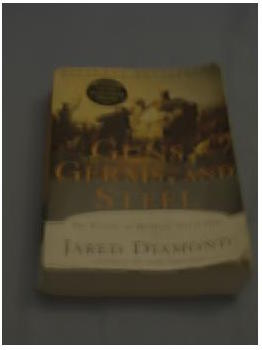
\includegraphics[width=1\linewidth]{book_deblurred} 
%\caption{Caption1}
%\label{fig:subim1}
%\end{wrapfigure}




\begin{figure*} [t]
\begin{center}
\graphicspath{ {deblursun/} }
\begin{subfigure}{0.32\textwidth}

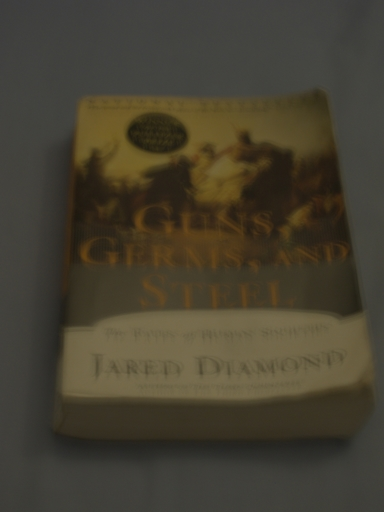
\includegraphics[width=0.9\linewidth]{book_s01_it0000_blurry} 
\caption{Blurry book image}
\label{fig:subim1}
\end{subfigure}
\begin{subfigure}{0.33\textwidth}
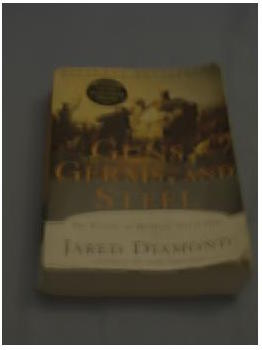
\includegraphics[width=0.9\linewidth]{book_deblurred}
\caption{Sun \etal (2015) result}
\label{fig:subim2}
\end{subfigure}
\begin{subfigure}{0.33\textwidth}
\graphicspath{ {deblurwhyte/} }
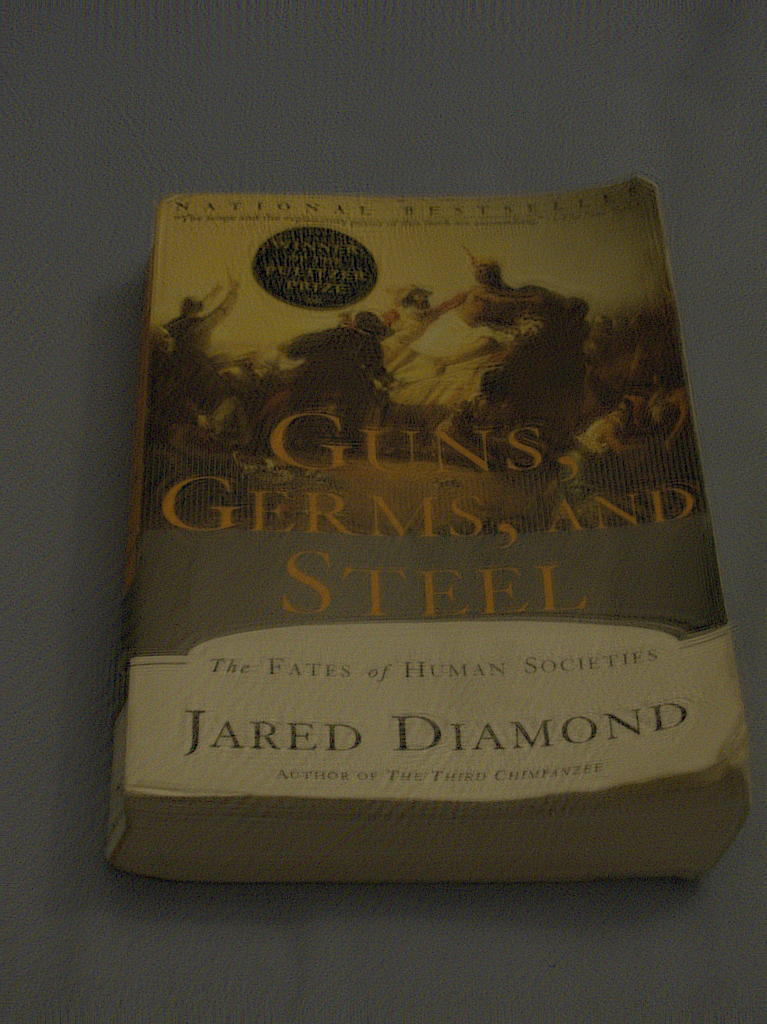
\includegraphics[width=0.9\linewidth]{book_whyte}
\caption{Whyte \etal (2012) result}
\label{fig:subim3}
\end{subfigure}
 
\caption{Blurry book image and deblurring results of the two algorithms}
\label{fig:image1}
\end{center}
\end{figure*}

\begin{figure*}
\begin{center}
\graphicspath{ {deblursun/} }
\begin{subfigure}{0.33\textwidth}

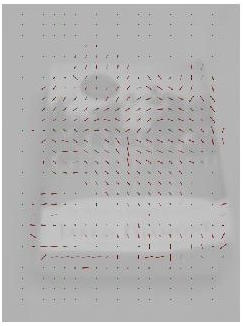
\includegraphics[width=0.9\linewidth]{book_kernels} 
\caption{Sun \etal (2015) kernels}
\label{fig:subim1}
\end{subfigure}
\begin{subfigure}{0.58\textwidth}
\graphicspath{ {deblurwhyte/} }
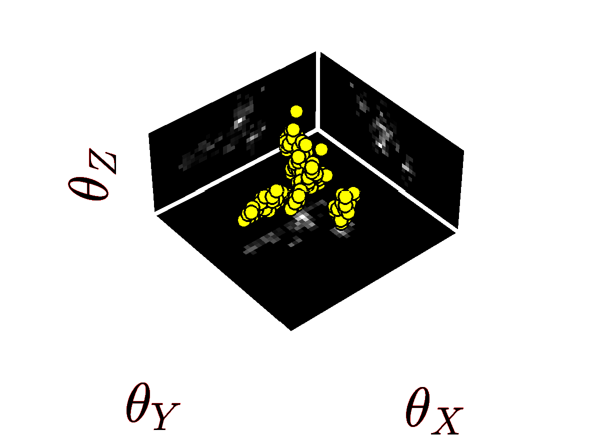
\includegraphics[width=0.9\linewidth]{book_kernel}
\caption{Whyte \etal (2012) 3D kernel}
\label{fig:subim3}
\end{subfigure}
 
\caption{Blur kernels associated with the two algorithms. Note that the Whyte \etal (2012) kernel is a 3D kernel and the Sun \etal (2015) set of kernels are 2D ones. This is the main difference Whyte \etal (2012) differs from the rest of the algorithms. Whyte \etal (2012)'s approach seems to be a better fit where the movement is more complex and cannot be expressed with simple movements as in Sun \etal (2015).}
\label{fig:image2}
\end{center}
\end{figure*}

\begin{figure*}
\begin{center}
\graphicspath{ {deblursun/} }
\begin{subfigure}{0.23\textwidth}

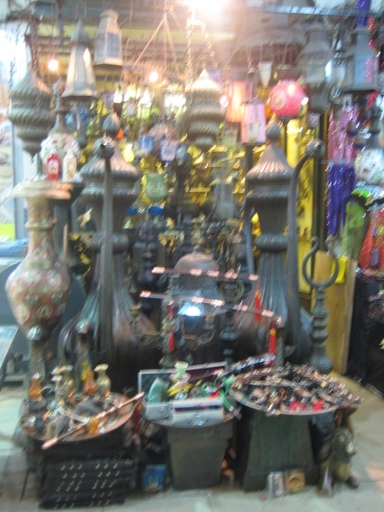
\includegraphics[width=0.9\linewidth]{istanbul_s01_it0000_blurry} 
\caption{Blurry image from Istanbul}
\label{fig:subim4}
\end{subfigure}
\begin{subfigure}{0.23\textwidth}
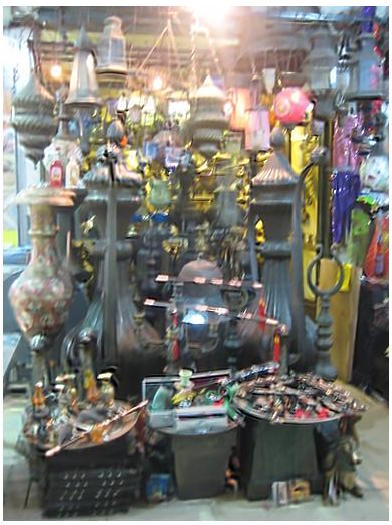
\includegraphics[width=0.9\linewidth]{istanbul_deblurred}
\caption{Sun \etal (2015) result}
\label{fig:subim5}
\end{subfigure}
\begin{subfigure}{0.23\textwidth}
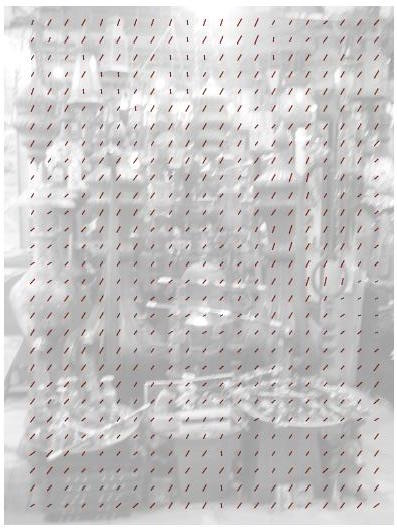
\includegraphics[width=0.9\linewidth]{istanbul_kernels}
\caption{Sun \etal (2015) kernels}
\label{fig:subim7}
\end{subfigure}
\begin{subfigure}{0.23\textwidth}
\graphicspath{ {deblurwhyte/} }
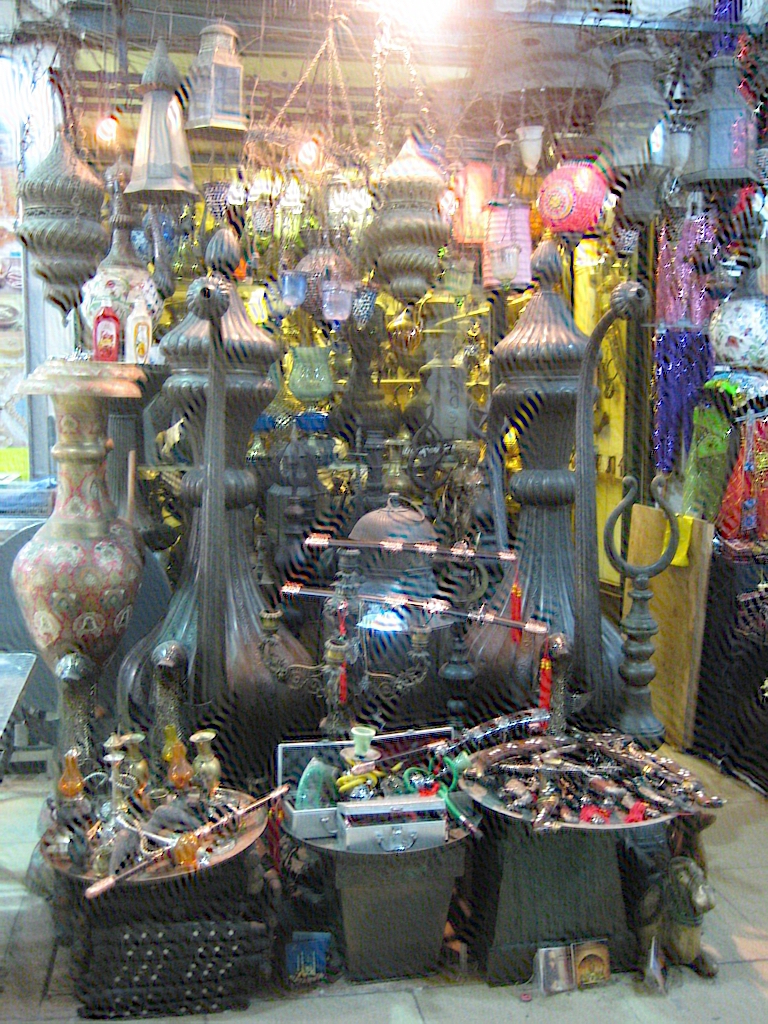
\includegraphics[width=0.9\linewidth]{istanbul_whyte}
\caption{Whyte \etal (2012) result}
\label{fig:subim6}
\end{subfigure}
 
\caption{Blurry image from Istanbul and deblurring results of the two algorithms. Whyte \etal (2012) has a lot of ringing effects because of saturation. Ringing is not so obvious for Sun \etal (2015).}
\label{fig:image3}
\end{center}
\end{figure*}

\begin{figure*}
\begin{center}
\graphicspath{ {deblursun/} }
\begin{subfigure}{0.45\textwidth}

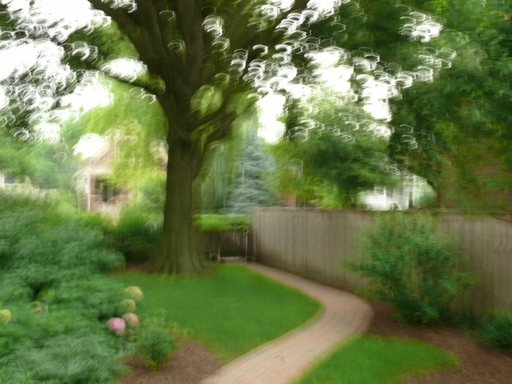
\includegraphics[width=0.9\linewidth]{garden_s01_it0000_blurry} 
\caption{Blurry image of a garden}
\label{fig:subim85}
\end{subfigure}
\begin{subfigure}{0.45\textwidth}
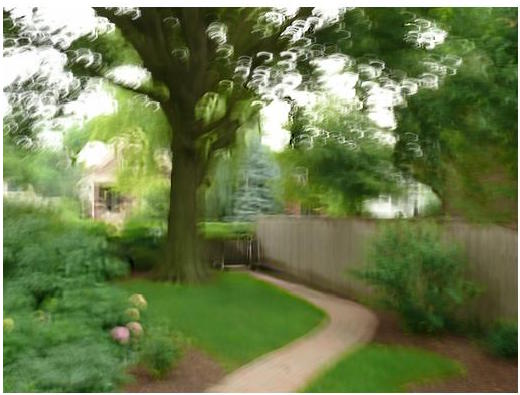
\includegraphics[width=0.9\linewidth]{garden_deblurred}
\caption{Sun \etal (2015) result}
\label{fig:subim86}
\end{subfigure}
\begin{subfigure}{0.45\textwidth}
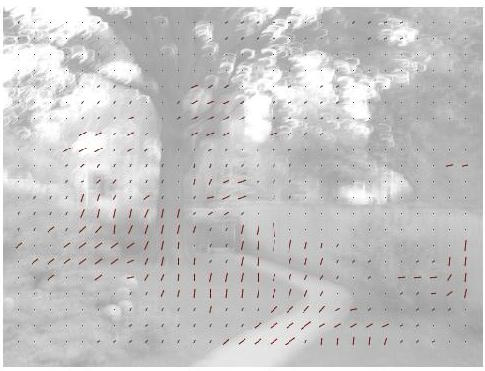
\includegraphics[width=0.9\linewidth]{garden_kernels}
\caption{Sun \etal (2015) kernels}
\label{fig:subim7}
\end{subfigure}
\begin{subfigure}{0.45\textwidth}
\graphicspath{ {deblurwhyte/} }
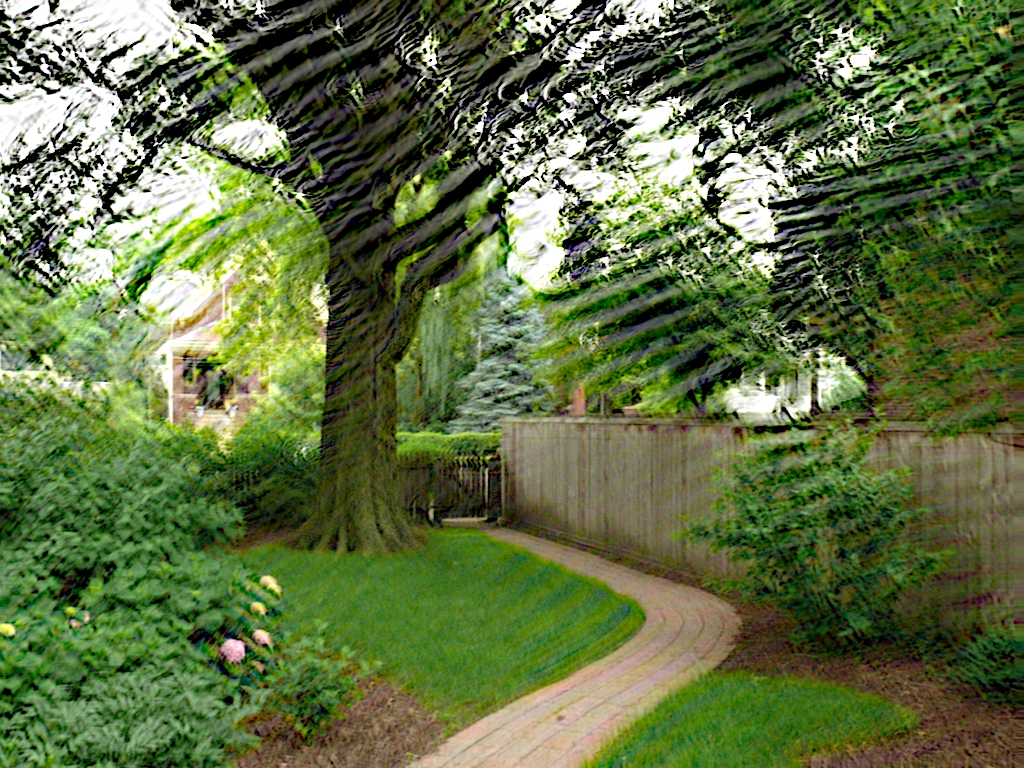
\includegraphics[width=0.9\linewidth]{garden_whyte}
\caption{Whyte \etal (2012) result}
\label{fig:subim6}
\end{subfigure}
 
\caption{Blurry image of a garden and deblurring results of the two algorithms. Whyte seems to be much more successful but might get a lower score in no-reference metric because of the ringing effects.}
\label{fig:image3}
\end{center}
\end{figure*}

\begin{figure*}
\begin{center}
\graphicspath{ {deblursun/} }
\begin{subfigure}{0.45\textwidth}

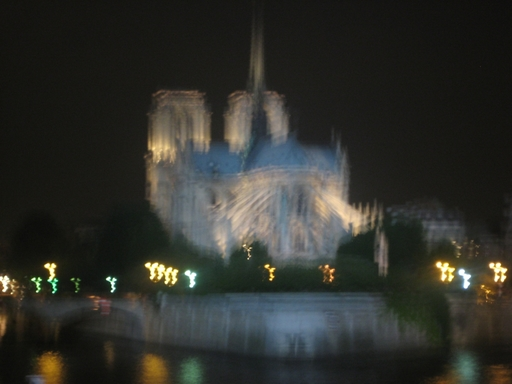
\includegraphics[width=0.9\linewidth]{notredame_s01_it0000_blurry} 
\caption{Blurry image from Notre Dame}
\label{fig:subim95}
\end{subfigure}
\begin{subfigure}{0.45\textwidth}
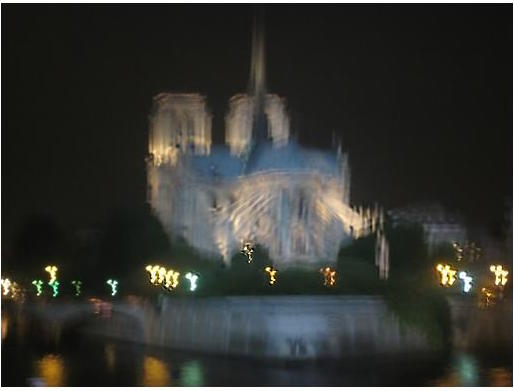
\includegraphics[width=0.9\linewidth]{notredame_deblurred}
\caption{Sun \etal (2015) result}
\label{fig:subim105}
\end{subfigure}
\begin{subfigure}{0.45\textwidth}
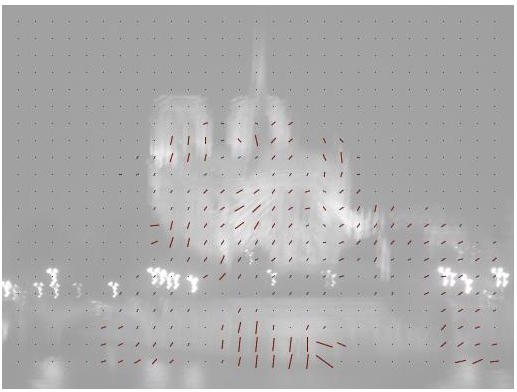
\includegraphics[width=0.9\linewidth]{notredame_kernels}
\caption{Sun \etal (2015) kernels}
\label{fig:subim7}
\end{subfigure}
\begin{subfigure}{0.45\textwidth}
\graphicspath{ {deblurwhyte/} }
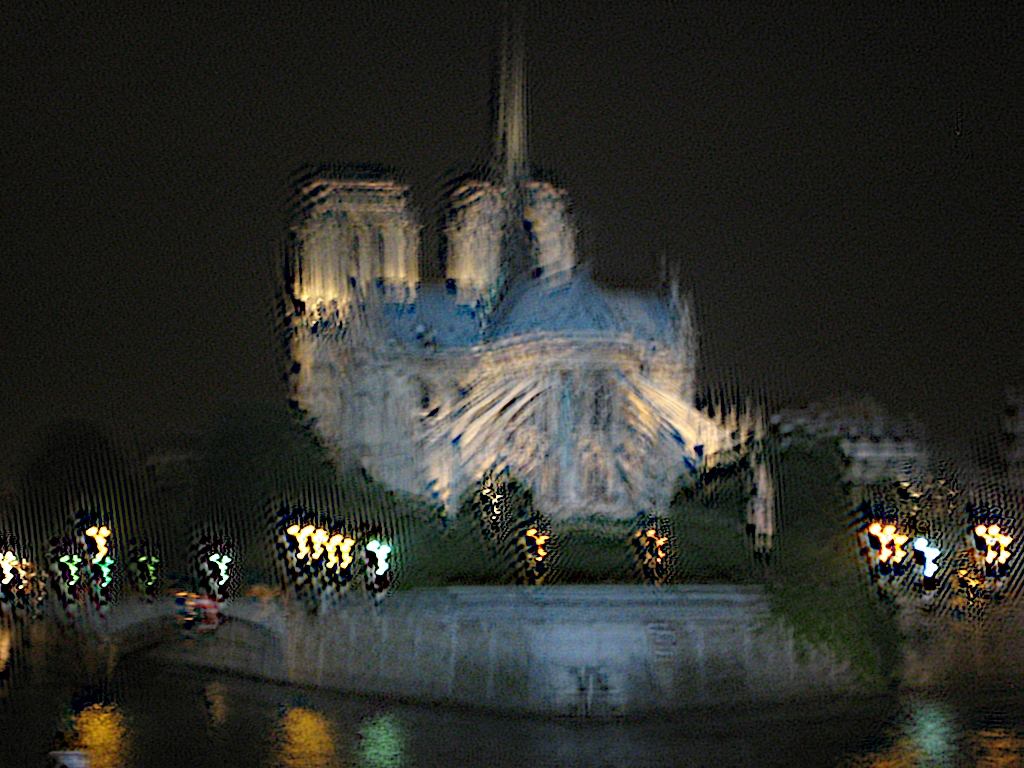
\includegraphics[width=0.9\linewidth]{notredame_whyte}
\caption{Whyte \etal (2012) result}
\label{fig:subim6}
\end{subfigure}
 
\caption{Blurry image from Notre Dame and deblurring results of the two algorithms. Sun \etal (2015) finds some kernels but the smoothness is not what a normal camera motion is expected to produce.}
\label{fig:image3}
\end{center}
\end{figure*}


%\begin{figure*}
%\begin{center}
%\graphicspath{ {deblursun/} }
%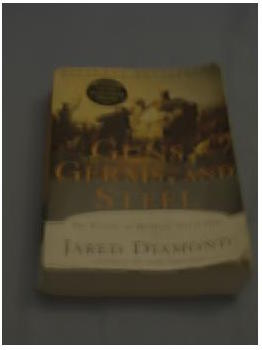
\includegraphics[width=0.4\linewidth]{book_deblurred}
%\caption{A caption}
%\end{center}
%\end{figure*}


\section{Conclusions}
In this study, we analyzed and evaluated two of the deblurring studies in the current literature. We evaluated the results using a recently developed metric that was designed to measure motion deblurring specifically, along with more traditional PSNR. The results show that neither of the deblurring techniques is the panacea of the blind motion deblurring problem. Both techniques are good for certain types of blurry pictures. Whyte \etal (2012) is no good for artifacts that arise after deblurring. Sun \etal (2015) cannot handle the problems with more complex motion types. Another interesting observation is that although visually more pleasing, some of the resulting images got low no-reference metric scores because of the ringing effects. Lastly there is no notable correlation between PSNR and no-reference metrics. The two metrics had a negative correlation for one metric and positive correlation across the two studies' results.



{\small
\bibliographystyle{ieee}
\bibliography{egbib}
}

\end{document}
